
%(BEGIN_QUESTION)
% Copyright 2007, Tony R. Kuphaldt, released under the Creative Commons Attribution License (v 1.0)
% This means you may do almost anything with this work of mine, so long as you give me proper credit

Examine this P\&ID:

$$\includegraphics[width=15.5cm]{i01658x01.eps}$$

Each pump is of the ``reciprocating'' type, a form of positive displacement machine.  In essence, each rotation of the motor shaft causes the pump to move a measured quantity of liquid from its inlet to its outlet.

What will happen to the liquid level inside the vessel over time if one pump is moving more liquid flow?
 
\vskip 10pt

Would you characterize this process as inherently {\it self-regulating} or inherently {\it integrating}?

\underbar{file i01658}
%(END_QUESTION)





%(BEGIN_ANSWER)

The liquid level inside the vessel will drift either up or down (depending on which pump moves more liquid) at a rate determined by the differential liquid flow ($Q_{in}$ $-$ $Q_{out}$).  This makes it an {\it integrating} process.

\vskip 10pt

Integrating processes are characterized by the capacity to experience persistent mass and/or energy imbalances, where the out-flow of mass and/or energy does not naturally reach equilibrium the in-flow over time.  Self-regulating processes, by contrast, naturally equalize their mass and energy balances as the process variable changes.

%(END_ANSWER)





%(BEGIN_NOTES)


%INDEX% Control, process characteristics: self-regulating versus integrating

%(END_NOTES)


